%=========================================================
% Geometric sheaf visualization on a 2D manifold (surface)
% U = union of coordinate patches, overlaps, and sections
%=========================================================
\documentclass[tikz,border=6pt]{standalone}
\usepackage{tikz}
\usetikzlibrary{arrows.meta,positioning,calc,decorations.pathreplacing,fit}

\usepackage{amssymb,amsmath}
\newcommand{\ord}{\operatorname{ord}}

\begin{document}
	
	%---------------------------------------------------------
	% Figure A: Manifold with open sets (patches) and overlaps
	%---------------------------------------------------------
	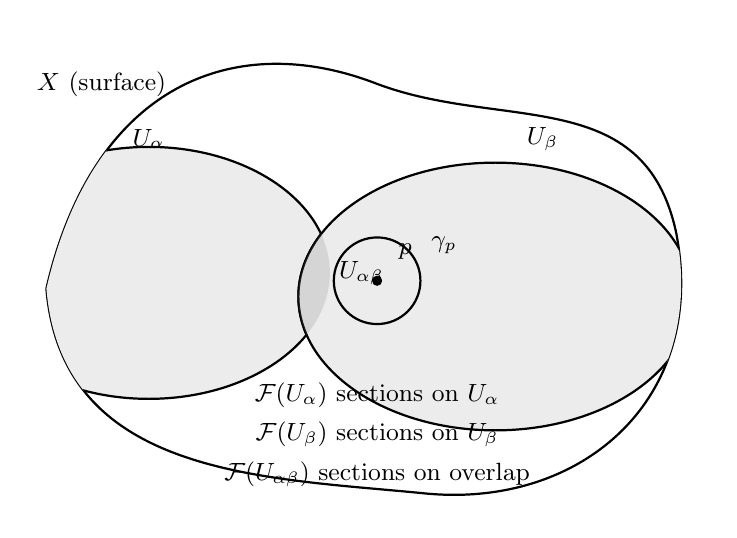
\begin{tikzpicture}[
		lab/.style={font=\small},
		arr/.style={-Latex,thick},
		patch/.style={draw=black,fill=gray!15,thick},
		overlap/.style={fill=gray!35,draw=black,thick,opacity=0.85},
		dot/.style={circle,fill=black,inner sep=1.3pt}
		]
		
		% --- "Manifold" outline (a blob)
		\draw[thick] (-4,0)
		.. controls (-3.4,2.6) and (-1.6,3.3) .. (0.2,2.6)
		.. controls (1.8,2.0) and (3.6,2.6) .. (4.0,0.7)
		.. controls (4.4,-1.4) and (2.8,-2.8) .. (0.8,-2.6)
		.. controls (-1.2,-2.4) and (-3.8,-2.4) .. (-4,0) -- cycle;
		
		\node[lab] at (-3.3,2.6) {$X$ (surface)};
		
		% --- Two open sets U_alpha, U_beta as "patches" on X
		\begin{scope}
			\clip (-4,0)
			.. controls (-3.4,2.6) and (-1.6,3.3) .. (0.2,2.6)
			.. controls (1.8,2.0) and (3.6,2.6) .. (4.0,0.7)
			.. controls (4.4,-1.4) and (2.8,-2.8) .. (0.8,-2.6)
			.. controls (-1.2,-2.4) and (-3.8,-2.4) .. (-4,0) -- cycle;
			
			% Patch U_alpha
			\filldraw[patch] (-2.7,0.2) ellipse (2.3 and 1.6);
			
			% Patch U_beta
			\filldraw[patch] (1.7,-0.1) ellipse (2.5 and 1.7);
			
			% Overlap shading (hand-drawn lens region)
			\begin{scope}
				\clip (-2.7,0.2) ellipse (2.3 and 1.6);
				\filldraw[overlap] (1.7,-0.1) ellipse (2.5 and 1.7);
			\end{scope}
		\end{scope}
		
		\node[lab] at (-2.7,1.9) {$U_\alpha$};
		\node[lab] at (2.3,1.9) {$U_\beta$};
		\node[lab] at (0.0,0.2) {$U_{\alpha\beta}$};
		
		% --- Mark a point p and a small loop gamma around it
		\node[dot] (p) at (0.2,0.1) {};
		\node[lab,above right=1mm and 1mm of p] {$p$};
		
		\draw[thick] (0.2,0.1) circle (0.55);
		\node[lab] at (1.05,0.55) {$\gamma_p$};
		
		% --- Labels about "sections over opens"
		\node[lab,below=11mm of p] {$\mathcal F(U_\alpha)$ sections on $U_\alpha$};
		\node[lab,below=16mm of p] {$\mathcal F(U_\beta)$ sections on $U_\beta$};
		\node[lab,below=21mm of p] {$\mathcal F(U_{\alpha\beta})$ sections on overlap};
		
	\end{tikzpicture}
	
	\vspace{8mm}
	
	%---------------------------------------------------------
	% Figure B: Gluing picture (local sections that agree on overlaps)
	%---------------------------------------------------------
	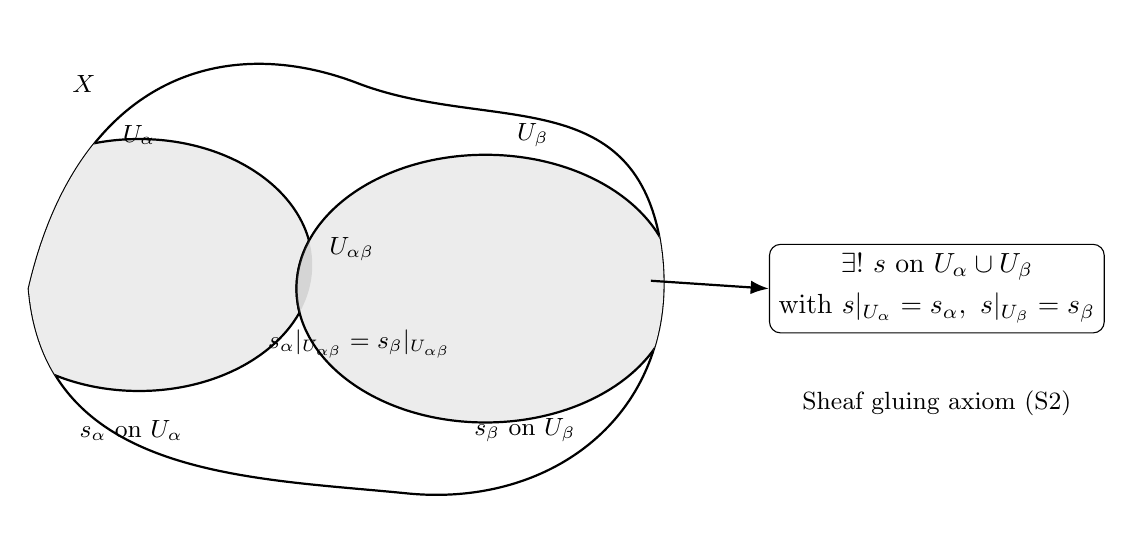
\begin{tikzpicture}[
		lab/.style={font=\small},
		arr/.style={-Latex,thick},
		patch/.style={draw=black,fill=gray!15,thick},
		overlap/.style={fill=gray!35,draw=black,thick,opacity=0.85},
		dot/.style={circle,fill=black,inner sep=1.3pt},
		box/.style={draw,rounded corners,minimum width=30mm,minimum height=9mm,align=center}
		]
		
		% --- Manifold outline (smaller)
		\draw[thick] (-4,0)
		.. controls (-3.4,2.6) and (-1.6,3.3) .. (0.2,2.6)
		.. controls (1.8,2.0) and (3.6,2.6) .. (4.0,0.7)
		.. controls (4.4,-1.4) and (2.8,-2.8) .. (0.8,-2.6)
		.. controls (-1.2,-2.4) and (-3.8,-2.4) .. (-4,0) -- cycle;
		
		\node[lab] at (-3.3,2.6) {$X$};
		
		\begin{scope}
			\clip (-4,0)
			.. controls (-3.4,2.6) and (-1.6,3.3) .. (0.2,2.6)
			.. controls (1.8,2.0) and (3.6,2.6) .. (4.0,0.7)
			.. controls (4.4,-1.4) and (2.8,-2.8) .. (0.8,-2.6)
			.. controls (-1.2,-2.4) and (-3.8,-2.4) .. (-4,0) -- cycle;
			
			\filldraw[patch] (-2.6,0.3) ellipse (2.2 and 1.6);
			\filldraw[patch] (1.8,0.0) ellipse (2.4 and 1.7);
			\begin{scope}
				\clip (-2.6,0.3) ellipse (2.2 and 1.6);
				\filldraw[overlap] (1.8,0.0) ellipse (2.4 and 1.7);
			\end{scope}
		\end{scope}
		
		\node[lab] at (-2.6,1.95) {$U_\alpha$};
		\node[lab] at (2.4,1.95) {$U_\beta$};
		\node[lab] at (0.1,0.5) {$U_{\alpha\beta}$};
		
		% --- Local sections (conceptual)
		\node[lab] at (-2.7,-1.8) {$s_\alpha$ on $U_\alpha$};
		\node[lab] at (2.3,-1.8) {$s_\beta$ on $U_\beta$};
		\node[lab] at (0.2,-0.7) {$s_\alpha|_{U_{\alpha\beta}}=s_\beta|_{U_{\alpha\beta}}$};
		
		% --- Arrow to glued section box
		\node[box,right=14mm of {(4,0)}] (glue) {$\exists!\ s\text{ on }U_\alpha\cup U_\beta$\\[1mm]
			$\text{with }s|_{U_\alpha}=s_\alpha,\ s|_{U_\beta}=s_\beta$};
		\draw[arr] (3.9,0.1) -- (glue.west);
		
		\node[lab,below=6mm of glue] {Sheaf gluing axiom (S2)};
		
	\end{tikzpicture}
	
	\vspace{8mm}
	
	%---------------------------------------------------------
	% Figure C: Specialize to O_X(D): "allowed poles" visualization
	%---------------------------------------------------------
	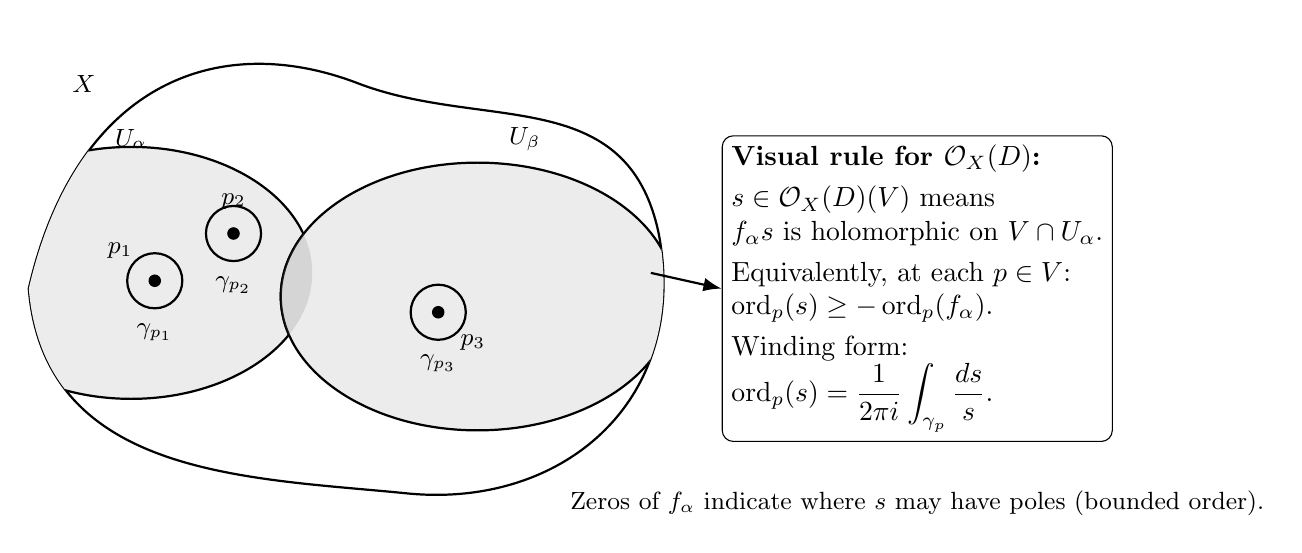
\begin{tikzpicture}[
		lab/.style={font=\small},
		arr/.style={-Latex,thick},
		patch/.style={draw=black,fill=gray!15,thick},
		overlap/.style={fill=gray!35,draw=black,thick,opacity=0.85},
		dot/.style={circle,fill=black,inner sep=1.3pt},
		pole/.style={circle,fill=black,inner sep=1.6pt},
		box/.style={draw,rounded corners,minimum width=45mm,minimum height=10mm,align=left}
		]
		
		% --- Manifold outline
		\draw[thick] (-4,0)
		.. controls (-3.4,2.6) and (-1.6,3.3) .. (0.2,2.6)
		.. controls (1.8,2.0) and (3.6,2.6) .. (4.0,0.7)
		.. controls (4.4,-1.4) and (2.8,-2.8) .. (0.8,-2.6)
		.. controls (-1.2,-2.4) and (-3.8,-2.4) .. (-4,0) -- cycle;
		
		\node[lab] at (-3.3,2.6) {$X$};
		
		\begin{scope}
			\clip (-4,0)
			.. controls (-3.4,2.6) and (-1.6,3.3) .. (0.2,2.6)
			.. controls (1.8,2.0) and (3.6,2.6) .. (4.0,0.7)
			.. controls (4.4,-1.4) and (2.8,-2.8) .. (0.8,-2.6)
			.. controls (-1.2,-2.4) and (-3.8,-2.4) .. (-4,0) -- cycle;
			
			\filldraw[patch] (-2.7,0.2) ellipse (2.3 and 1.6);
			\filldraw[patch] (1.7,-0.1) ellipse (2.5 and 1.7);
			\begin{scope}
				\clip (-2.7,0.2) ellipse (2.3 and 1.6);
				\filldraw[overlap] (1.7,-0.1) ellipse (2.5 and 1.7);
			\end{scope}
		\end{scope}
		
		\node[lab] at (-2.7,1.9) {$U_\alpha$};
		\node[lab] at (2.3,1.9) {$U_\beta$};
		
		% --- Mark points where f_alpha has zeros (so s may have poles there)
		\node[pole] (z1) at (-2.4,0.1) {};
		\node[pole] (z2) at (-1.4,0.7) {};
		\node[pole] (z3) at (1.2,-0.3) {};
		\node[lab,above left=1mm and 1mm of z1] {$p_1$};
		\node[lab,above=1mm of z2] {$p_2$};
		\node[lab,below right=1mm and 1mm of z3] {$p_3$};
		
		% --- small loops around these points (to suggest winding/order)
		\draw[thick] (-2.4,0.1) circle (0.35);
		\draw[thick] (-1.4,0.7) circle (0.35);
		\draw[thick] (1.2,-0.3) circle (0.35);
		
		\node[lab] at (-2.4,-0.55) {$\gamma_{p_1}$};
		\node[lab] at (-1.4,0.05) {$\gamma_{p_2}$};
		\node[lab] at (1.2,-0.95) {$\gamma_{p_3}$};
		
		% --- Explanation box
		\node[box,right=8mm of {(4,0)}] (ex) {
			\textbf{Visual rule for $\mathcal O_X(D)$:}\\[1mm]
			$s\in\mathcal O_X(D)(V)$ means \\
			$f_\alpha s$ is holomorphic on $V\cap U_\alpha$.\\[1mm]
			Equivalently, at each $p\in V$: \\
			$\ord_p(s)\ge -\ord_p(f_\alpha)$.\\[1mm]
			Winding form: \\
			$\displaystyle \ord_p(s)=\frac{1}{2\pi i}\int_{\gamma_p}\frac{ds}{s}$.
		};
		\draw[arr] (3.9,0.2) -- (ex.west);
		
		\node[lab,below=5mm of ex] {Zeros of $f_\alpha$ indicate where $s$ may have poles (bounded order).};
		
	\end{tikzpicture}
	
\end{document}
